
% \section{Rossby-Wellen}
\begin{frame}{Rossby-Wellen auf der Kugel}
    \begin{columns}
      \column{0.55\textwidth}
      \begin{itemize}
        \item Idealisierte Strömung basierend auf der \textbf{Stromfunktion}:
        \[
          \psi(\theta, \phi) = \hat{\psi} \cos(k \phi) \sin(\theta)
        \]
        \item Daraus ergibt sich das Geschwindigkeitsfeld über:
        \[
          u = -\frac{1}{a} \frac{\partial \psi}{\partial \theta}, \quad
          v = \frac{1}{a \sin \theta} \frac{\partial \psi}{\partial \phi}
        \]
        \item Wellenzahl \( k \), mittlerer Wind \( U_0 \), \\
              Erdradius \( a \), Beta-Effekt implizit enthalten
        \item Die Westwärts-Drift ist charakteristisch für Rossby-Wellen
      \end{itemize}
  
      \column{0.45\textwidth}
      \centering
      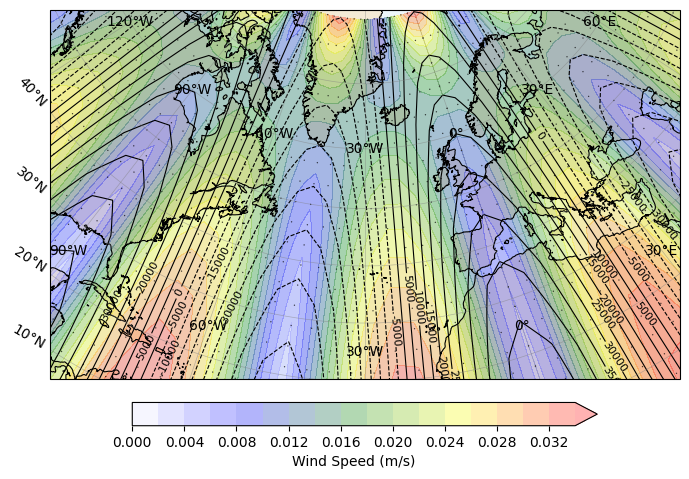
\includegraphics[width=\linewidth]{../images/rossby_wave_plot.png}
    \end{columns}
  \end{frame}
  
  \begin{frame}{Rossby-Wellen auf der  $\beta$-Ebene}
    \begin{columns}
      \column{0.55\textwidth}
      \begin{itemize}
        \item Lineare Lösung der barotropen Vorticity-Gleichung auf der $\beta$-Ebene:
        \[
          \frac{\partial}{\partial t} \left( \nabla^2 \psi \right) + \beta \frac{\partial \psi}{\partial x} = 0
        \]
        \item Wellenansatz für die Stromfunktion:
        \[
          \psi(x, y, t) = \hat{\psi} \cos(kx + ly - \omega t)
        \]
        \item Dispersionsrelation:
        \[
          \omega = -\beta \frac{k}{k^2 + l^2}
        \]
        \item Geschwindigkeit:
        \[
          u = -\frac{\partial \psi}{\partial y}, \quad
          v = \frac{\partial \psi}{\partial x}
        \]
        \item Charakteristisch: westwärts laufende Phasengeschwindigkeit bei \( \beta > 0 \)
      \end{itemize}
  
      \column{0.45\textwidth}
      \centering
      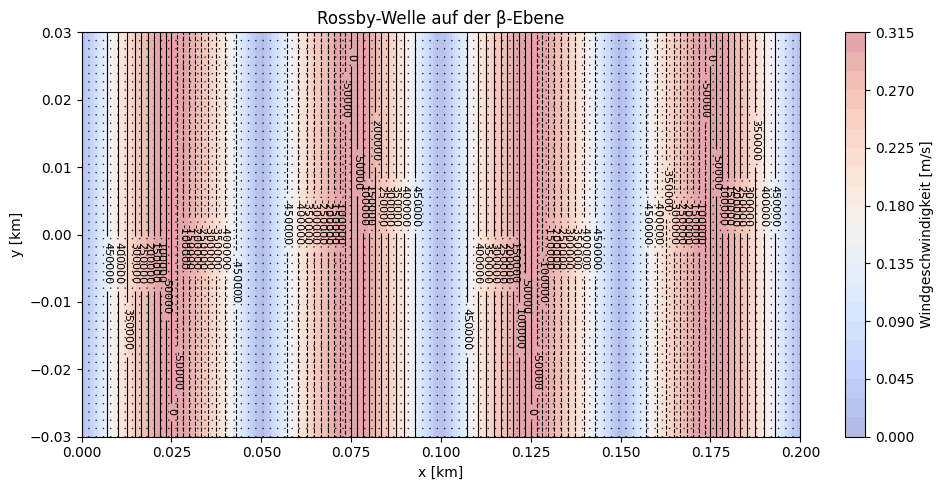
\includegraphics[width=\linewidth]{../images/rossby_wave_beta.png}
      \scriptsize Darstellung: Windvektoren (Pfeile), Stromfunktion (schwarz), Windgeschwindigkeit (Farbflächen)
    \end{columns}
  \end{frame}
  